\documentclass{article}
\usepackage{tikz}

\begin{document}

\begin{figure}[h]
    \centering
    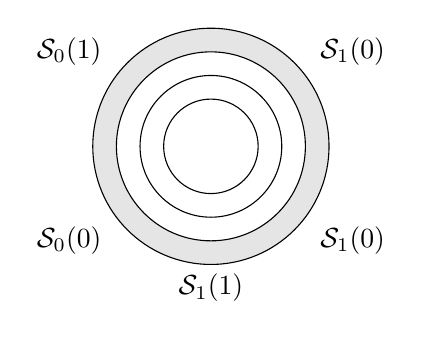
\begin{tikzpicture}[scale=1.5]

        % Draw the circles
        \draw[fill=gray!20] (0,0) circle (1);
        \draw[fill=white] (0,0) circle (0.8);
        \draw[fill=white] (0,0) circle (0.6);
        \draw[fill=white] (0,0) circle (0.4);

        % Draw the labels
        \node at (-1.2, 0.8) {$\mathcal{S}_0(1)$};
        \node at (1.2, 0.8) {$\mathcal{S}_1(0)$};
        \node at (-1.2, -0.8) {$\mathcal{S}_0(0)$};
        \node at (1.2, -0.8) {$\mathcal{S}_1(0)$};
        \node at (0, -1.2) {$\mathcal{S}_1(1)$};

    \end{tikzpicture}
\end{figure}

\begin{figure}[h]
    \centering
    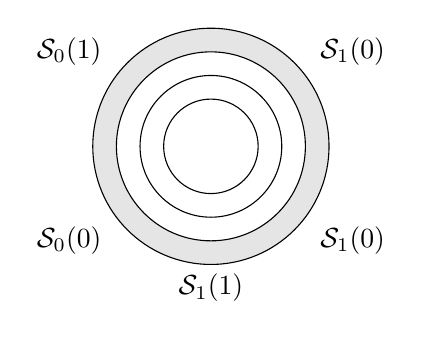
\begin{tikzpicture}[scale=1.5]

        % Draw the circles
        \draw[fill=gray!20] (0,0) circle (1);
        \draw[fill=white] (0,0) circle (0.8);
        \draw[fill=white] (0,0) circle (0.6);
        \draw[fill=white] (0,0) circle (0.4);

        % Draw the labels
        \node at (-1.2, 0.8) {$\mathcal{S}_0(1)$};
        \node at (1.2, 0.8) {$\mathcal{S}_1(0)$};
        \node at (-1.2, -0.8) {$\mathcal{S}_0(0)$};
        \node at (1.2, -0.8) {$\mathcal{S}_1(0)$};
        \node at (0, -1.2) {$\mathcal{S}_1(1)$};

    \end{tikzpicture}
\end{figure}

\end{document}